\documentclass[aspectratio=169,11pt]{beamer}
\usepackage{luatexja}
\usepackage[haranoaji]{luatexja-preset}
\usepackage{amsmath,amssymb,bm}
\usepackage{subcaption}

\usetheme{Madrid}
\usecolortheme{seahorse}

\title{事後分布の例：混合正規分布モデル}
\subtitle{特異学習理論入門 第1章}
\author{Shiryu Nakano}
\date{\today}

\AtBeginSection[]{
  \begin{frame}{目次}
    \tableofcontents[currentsection]
  \end{frame}
}

\begin{document}
\frame{\titlepage}

\begin{frame}{目次}
  \tableofcontents
\end{frame}

\section{事後分布の例}

% --- スライド2: モデルの定義 ---
\begin{frame}{モデルの定義}
  $x \in \mathbb{R}^1$ とし，$\mathcal{N}(x)$ を標準正規分布とする：
  \begin{equation*}
    \mathcal{N}(x) = \frac{1}{\sqrt{2\pi}} \exp\!\left(-\frac{x^2}{2}\right)
  \end{equation*}

  パラメータ $w = (a,\, b)$ をもつ\textbf{混合正規分布モデル}：
  \begin{equation*}
    p(x \mid w) = (1-a)\,\mathcal{N}(x) + a\,\mathcal{N}(x - b)
  \end{equation*}

  \begin{itemize}
    \item $0 \leqq a \leqq 1$，$b \in \mathbb{R}^1$
    \item 2つの正規分布の重み付き和
  \end{itemize}
\end{frame}

% --- スライド3: 実験設定 ---
\begin{frame}{実験設定}
  \begin{columns}[T]
    \begin{column}{0.5\textwidth}
      \textbf{パラメータ空間・事前分布}
      \begin{align*}
        W &= \{(a,b) \mid 0 \leqq a \leqq 1,\ |b| \leqq 5\} \\[4pt]
        \varphi(w) &= \frac{1}{10} \quad \text{（一様事前分布）}
      \end{align*}
      \vspace{0.5em}
      事後分布 $\approx$ 尤度関数\\
      （最尤推定量 $=$ MAP推定量）
    \end{column}
    \begin{column}{0.5\textwidth}
      \textbf{真のパラメータ（3通り）}
      \begin{equation*}
        (a_0,\, b_0) =
        \begin{cases}
          (0.5,\ 3.0) \\[4pt]
          (0.5,\ 1.0) \\[4pt]
          (0.5,\ 0.5)
        \end{cases}
      \end{equation*}
      \vspace{0.5em}
      サンプル数 $n = 100$
    \end{column}
  \end{columns}
\end{frame}

% --- スライド4: 概観 ---
\begin{frame}{概観：3ケースの事後分布}
  \begin{figure}
    \centering
    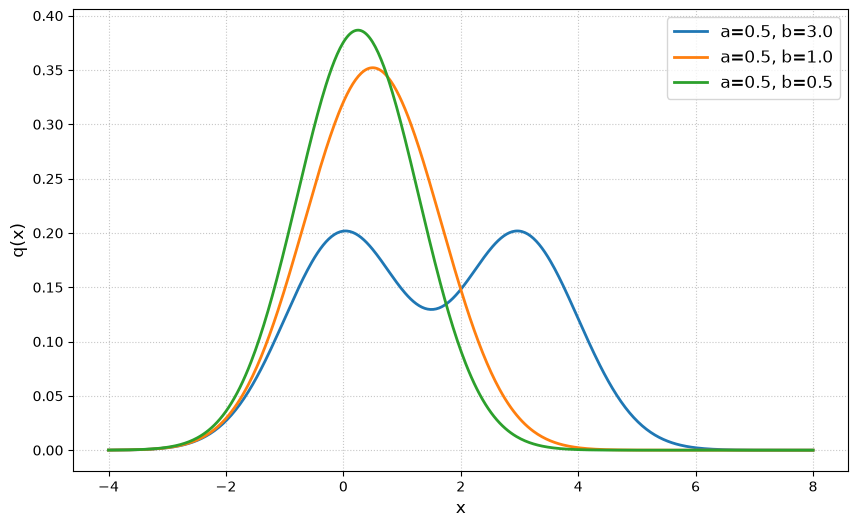
\includegraphics[width=0.55\linewidth,height=0.72\textheight,keepaspectratio]{../figures/image-3.png}
    \caption{混合正規分布モデルの事後分布（$n=100$）}
  \end{figure}
\end{frame}

% --- スライド5: ケース(i) ---
\begin{frame}{ケース(i)：$(a_0,\, b_0) = (0.5,\ 3.0)$}
  \begin{columns}[T]
    \begin{column}{0.52\textwidth}
      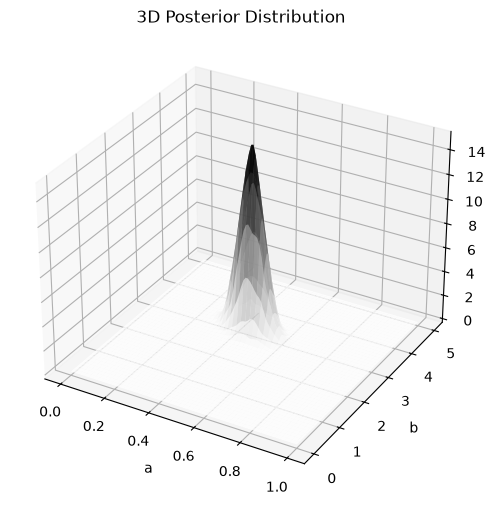
\includegraphics[width=\linewidth,height=0.75\textheight,keepaspectratio]{../figures/image-4.png}
    \end{column}
    \begin{column}{0.45\textwidth}
      \textbf{$b_0 = 3.0$：2分布が十分に離れている}
      \begin{itemize}
        \item $n=100$ で2つの正規分布の混合と明確に判別可能
        \item 事後分布は真のパラメータ付近に\textbf{鋭いピーク}
        \item 正規分布で近似できる
        \item 最尤推定量：$(0.47,\, 3.05)$（真値に近い）
        \item サンプルの出方への依存が小さい
      \end{itemize}
    \end{column}
  \end{columns}
\end{frame}

% --- スライド6: ケース(ii) ---
\begin{frame}{ケース(ii)：$(a_0,\, b_0) = (0.5,\ 1.0)$}
  \begin{columns}[T]
    \begin{column}{0.52\textwidth}
      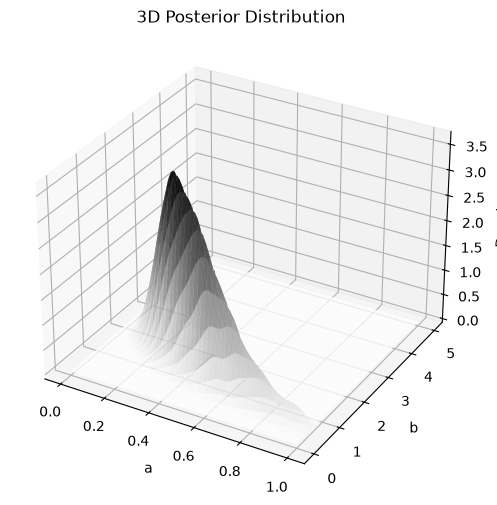
\includegraphics[width=\linewidth,height=0.75\textheight,keepaspectratio]{../figures/image-5.png}
    \end{column}
    \begin{column}{0.45\textwidth}
      \textbf{$b_0 = 1.0$：2分布が重なっている}
      \begin{itemize}
        \item $n=100$ では1つか2つかの判別が難しい場合あり
        \item 事後分布が真のパラメータからずれて\textbf{広がる}
        \item 正規分布では近似できない
        \item 最尤推定量：$(0.65,\, 0.55)$（真値からずれ）
        \item サンプルの出方で位置・形状が変化
      \end{itemize}
    \end{column}
  \end{columns}
\end{frame}

% --- スライド7: ケース(iii) ---
\begin{frame}{ケース(iii)：$(a_0,\, b_0) = (0.5,\ 0.5)$}
  \begin{columns}[T]
    \begin{column}{0.52\textwidth}
      
\includegraphics[width=\linewidth,height=0.75\textheight,keepaspectratio]{../figures/image.png}
    \end{column}
    \begin{column}{0.45\textwidth}
      \textbf{$b_0 = 0.5$：2分布がほぼ一致}
      \begin{itemize}
        \item $n=100$ では1つの正規分布に見える
        \item 事後分布が $ab \approx 0$ を満たす集合全体に\textbf{大きく広がる}
        \item 正規分布では近似できない
        \item 最尤推定量：$(0.15,\, 0.71)$（真値 $(0.5, 0.5)$ と大きくずれ）
        \item サンプルの出方で形状が大きく変動
      \end{itemize}
    \end{column}
  \end{columns}
\end{frame}

% --- スライド8: 3ケースの比較 ---
\begin{frame}{3ケースの比較}
  \begin{figure}
    \centering
    \begin{subfigure}[b]{0.3\textwidth}
      \centering
      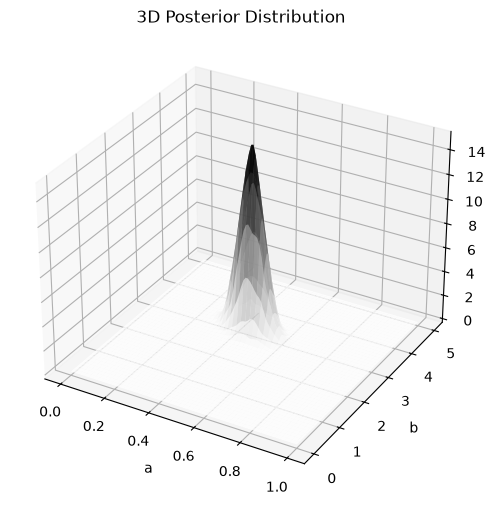
\includegraphics[width=\linewidth]{../figures/image-4.png}
      \caption{(i) $b_0 = 3.0$}
    \end{subfigure}
    \hfill
    \begin{subfigure}[b]{0.3\textwidth}
      \centering
      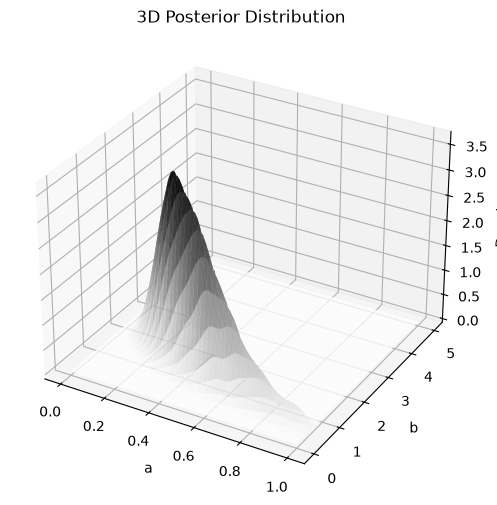
\includegraphics[width=\linewidth]{../figures/image-5.png}
      \caption{(ii) $b_0 = 1.0$}
    \end{subfigure}
    \hfill
    \begin{subfigure}[b]{0.3\textwidth}
      \centering
      
\includegraphics[width=\linewidth]{../figures/image.png}
      \caption{(iii) $b_0 = 0.5$}
    \end{subfigure}
    \caption{真のパラメータの違いによる事後分布の変化（$n=100$）}
  \end{figure}
\end{frame}


\if0
% --- スライド9: まとめ・示唆 ---
\begin{frame}{まとめ：示唆}
  \begin{block}{古典統計の仮定}
    事後分布が局所的に鋭いピークを持ち，正規分布で近似できる（ケース(i)）
  \end{block}

  \begin{alertblock}{現実・特異モデルでは}
    事後分布が大局的な広がりを持つことがある（ケース(ii), (iii)）
  \end{alertblock}

  \vspace{0.8em}
  \textbf{推測精度の比較}
  \begin{itemize}
    \item 正規近似できる場合：ベイズ・最尤・その他の推測がほぼ同精度
    \item 正規近似できない場合：\textbf{ベイズ推測が他の方法より優れる}
  \end{itemize}

  \vspace{0.8em}
  \textbf{本書の方針}
  \begin{itemize}
    \item 3章：正規近似できる場合の理論
    \item 4章：大局的な広がりを持つ場合でも扱える理論（特異学習理論）
  \end{itemize}
\end{frame}

\fi
\end{document}

